\documentclass{article}
\usepackage{spconf,amsmath,graphicx}
\usepackage{amssymb}
\usepackage{enumitem}
\usepackage{hyperref}

\title{Pruning Subsequence Search with Attention-Based Embedding}

\name{Colin Raffel and Daniel P. W. Ellis}
\address{LabROSA\\
    Columbia University\\
    New York, NY}

\begin{document}
\ninept
\maketitle

\begin{abstract}
Finding the most similar sequence to a query in a database of sequences can be prohibitively expensive when the database size is large.
Typically, the scalability of different approaches are dependent on various ``pruning'' techniques, which use heuristics to avoid expensive comparisons against a large subset of the database.
We present an approximate pruning technique which involves embedding sequences in a Euclidean space.
Sequences are embedded using a convolutional network with a form of attention which integrates over time, which is trained using matching and non-matching pairs of sequences.
By using fixed-length embeddings, our pruning method effectively runs in constant time, making it many orders of magnitude faster when compared to full Dynamic Time Warping-based matching.
We demonstrate the effectiveness of our approach on a large-scale musical score-to-audio recording retrieval task.
\end{abstract}

\begin{keywords}
Sequence Retrieval, Attention-Based Models, Convolutional Networks, Dynamic Time Warping, Pruning
\end{keywords}

\section{Introduction}
\label{sec:intro}

Sequences\footnote{In this work, we refer to ``signals'' by the slightly more generic term ``sequences'', but the two can be used interchangeably.} are a natural way of representing data in a wide range of fields, including multimedia, environmental sciences, natural language processing, and biology.
The proliferation of sensors and decreasing cost of storage in recent years has resulted in the creation of very large databases of sequences.
Given such a database, a fundamental task is to find the database entry which is most similar to a query.
However, this task can be prohibitively expensive depending on both the method used to compare sequences and the size of the database.

An effective way to compare sequences is the Dynamic Time Warping (DTW) distance, first proposed in the context of speech utterances \cite{sakoe1978dynamic}.
DTW first computes an optimal alignment of the two sequences of feature vectors being compared, and then reports their distance as the total distance among aligned feature vectors.
The alignment step makes DTW much more robust to phase or offset errors than typical distance metrics, such as the Euclidean distance \cite{rakthanmanon2012searching}.
DTW also naturally extends to the setting where subsequence matching is allowed.
Using dynamic programming, the optimal DTW alignment can be found in time quadratic in the length of the sequences.
Despite this optimization, naive application of DTW to nearest-neighbor retrieval of the most similar sequence in a database can be prohibitively expensive.
Other dynamic programming-based ``edit distance'' metrics are used when appropriate, and are similar in both their effectiveness and inefficiency.

To mitigate this issue, a variety of ``pruning methods'' have been proposed.
The idea behind these techniques is to use heuristics to avoid computing the full DTW alignment for a large proportion of the database.
\cite{rakthanmanon2012searching} gives a broad overview of different pruning methods, and shows that their application makes exact retrieval feasible in extremely large (e.g.\ trillions of sequences) databases.
However, these methods rely on various assumptions, including that the query sequence is a subsequence of its correct match and the length of the alignment path is known a priori.

An alternative approach is to replace the DTW search with a surrogate problem which is faster to solve.
For example, \cite{papapetrou2011embedding} proposes a technique which maps sequences to a fixed-length embedding, which avoids DTW calculation when matching the query to the database.
The embedding is constructed by pre-computing the DTW distance between each sequence in the database and a small collection of ``reference'' sequences, which are chosen to optimize retrieval accuracy.
Then, to match a query sequence to the database, its DTW distance is computed against the same collection of reference sequences, and the resulting vector of DTW distances is matched against the database of embeddings using a standard Euclidean distance-based nearest-neighbor search.
The resulting algorithm is approximate, but provided state-of-the-art rsults both in terms of accuracy and speed.
This technique relies on the same assumptions as the pruning methods described in \cite{rakthanmanon2012searching}.
In addition, it presents a trade-off between efficiency and accuracy where more reference sequences generally improve accuracy but require more full DTW calculations to be made, which can be prohibitively expensive for very long or very high-dimensional sequences.

In \cite{raffel2015large}, a more general approximate method is proposed where a neural network model is used to map and downsample sequences of feature vectors to shorter sequences of bit vectors.
Computing the distance between bit vectors can be achieved by a single exclusive-or operation followed by a table lookup, so this approach vastly improves the efficiency of the local distance calculations involved in DTW.
Furthermore, downsampling the sequences gives quadratic speed gains.
In an experiment matching transcriptions of musical pieces to audio recordings in a large database, using this method allowed for 99\% of the entries in the database to be pruned with high confidence.
However, this approach still relies on DTW which is quadratic-time and therefore provides room for efficiency improvements.

Motivated by the above issues, we propose a learning-based system for producing sequence embeddings for approximate matching.
Our approach is similar in spirit to \cite{papapetrou2011embedding}, except that it is fully general, i.e.\ it does not rely on any assumptions about the alignment length or whether the query is a subsequence of its match.
This is thanks to the fact that we utilize an attention-based neural network model which can adapt to any problem setting according to the training data provided.
Our approach is also constant-time: By mapping sequences to a fixed-length embedding, comparing a query to each database entry is a single Euclidean distance calculation, which does not become less efficient for longer or higher-dimensional sequences.

In the following section, we discuss embedding and attention-based neural network models, which we use to motivate our proposed model in Section \ref{sec:model}.
In Section \ref{sec:experiment}, we evaluate the effectiveness of our proposed model on the task of matching musical transcriptions to audio recordings of their corresponding songs in a large database.
Finally, we discuss results and possibilities for improvement in Section \ref{sec:results}.

\section{Embedding and Attention}
\label{sec:embedding}

The idea of ``embedding'' is an attractive one: Given data which is provided in a representation which is either inefficient or does not readily reveal factors of interest, can we produce a mapping to fixed-length vectors for which our data has the desired properties?
Because many simple machine learning methods are very effective given data where Euclidean distance corresponds to some notion of similarity, embedding can make data more amenable to learning and comparison.

As a concrete example, in \cite{schroff2015facenet}, a neural network architecture is used to embed images of faces such that images of the same person have small pairwise distances in the embedded space images of different people have large distances.
The authors were able to achieve state-of-the-art results on the ``labeled faces the wild'' dataset by simply thresholding the resulting distances to denote ``same person'' or ``different person''.
In addition, the embedded representation produced qualitatively useful results when performing unsupervised clustering using $k$-means.
Another highly effective application of embedding is word2vec, which is a family of models for mapping words to a Euclidean space which has desireable properties \cite{mikolov2013distributed}.
For example, the difference between ``China'' and ``Beijing'' in the embedded space is roughly equivalent to the difference between ``Rome'' and ``Italy''.

The idea of embedding has also been applied to sequences.
Notably, in \cite{sutskever2014sequence}, a recurrent network was trained to map a sequence of words in a source language to a fixed-length vector, which was then used to generate a sequence of words in a target language, resulting in a quality translation of the original sentence.
The resulting source-sentence embeddings encoded high-level linguistic characteristics, such as invariance to word order in sentences with the same meaning.
A benefit of using recurrent networks is their ability to summarize an entire sequence of arbitrary length as a fixed-length vector, which brings the possibility of learning embeddings to sequences.

One issue with using recurrent networks is their difficulty in modeling long-term dependencies \cite{bengio1994learning}.
In the embedding setting, this may result in the end of the sequence having more of an effect on the embedding than the beginning.
A recently proposed technique for mitigating this issue is ``attention'' \cite{bahdanau2014neural}.
Conceptually, an attention-based model includes a mechanism which learns to assign a weighing at each sequence step based on the current and all previous feature vectors.
When used with recurrent networks, the addition of attention has proven effective in a wide variety of domains including speech recognition, machine translation, and image captioning \cite{cho2015describing}.

At a high level, attention-based models are similar to the common technique of summarizing a sequence of feature vectors by the mean, variance, and occasionally covariance of feature dimensions.
This simple approach has seen frequent application in the domain of music information retrieval, where it has proven to be surprisingly effective at genre classification \cite{bergstra2006aggregate, tzanetakis2002musical}, instrument classification \cite{deng2008study}, artist recognition \cite{mandel2005song}, and similarity rating prediction \cite{foster2014sequential}.
Attention-based models can be seen as a generalization of this technique where both the feature representation and a weighted average are both optimized and data-adaptive.

\section{Feed-forward Attention}
\label{sec:model}

While previous work on attention-based models has focused on recurrent networks, in the present work we will use feed-forward networks for the following reasons:
First, Recurrent networks have difficulty modelling very long-term dependencies \cite{bengio1994learning}.
In the experiment described in Section \ref{sec:experiment}, sequences may have thousands of time steps, which is prohibitively long even for sophisticated models such as long short-term memory networks \cite{hochreiter1997long}.
Second, feed-forward networks are much more efficient to train and evaluate than recurrent networks because their operations can be completely parallelized, whereas recurrent networks must evaluate each time step sequentially.
Finally, attention provides its own form of temporal modelling due to the fact that it integrates over the entire sequence.
We therefore propose a ``feed-forward'' variant of attention, which computes a weighting for each sequence step independent of all other steps.

Our simplified variant of attention can be formulated as follows:
Given a matrix which comprises a sequence of $M$ $D$-dimensional vectors $X \in \mathbb{R}^{M \times D}$, we compute weights $\alpha \in \mathbb{R}^M$ using the following transformation:
\begin{equation}
\label{eq:alpha}
\alpha = \mathrm{softmax}(\sigma(Xw + b))
\end{equation}
where
$$
\mathrm{softmax}(x)_j = \frac{e^{x_j}}{\sum_{i = 1}^M e^{x_i}}
$$
and $\sigma$ is some nonlinear function (throughout this work, we will use $\sigma = \tanh$).
$w \in \mathbb{R}^D$ and $b \in \mathbb{R}$ are parameters of the transformation, which can be learned as part of a larger feed-forward network model.
After computing $\alpha$, the weighted average of the vectors in $X$ is computed by
$$
\hat{X} = \sum_{i = 1}^M \alpha_i X_{i, :}
$$
Conceptually, this attention mechanism can be thought of as using $w$, $b$, and $\sigma$ to compute scalar ``importance'' values for each vector in $X$, which are then normalized using the softmax function and used to compute a weighted mean $\hat{X}$ over all vectors in $X$.

The main difference between this formulation and the one proposed in \cite{bahdanau2014neural, cho2015describing} is that here we are only producing a single weighting $\alpha$ for the entire sequence rather than a different $\alpha$ at each time step.
This is primarily because our goal in embedding is to produce a single vector for the entire sequence whereas previous applications of attention have mainly focused on sequence-to-sequence transduction.
As a result, Equation \ref{eq:alpha} does not contain any terms for a previous attention vector or a previous hidden state, because in the present contexts these quantities do not exist.
The main disadvantage to using attention in this way is that it ignores temporal order by computing an average over the entire sequence.
However, motivated by the surprising effectiveness of the unweighted/non-adaptive Gaussian results discussed in Section \ref{sec:embedding}, we submit that this approach will be effective and verify its utility in the following section.

\section{Pruning Experiment}
\label{sec:experiment}

\begin{figure}[t]
  \centering
  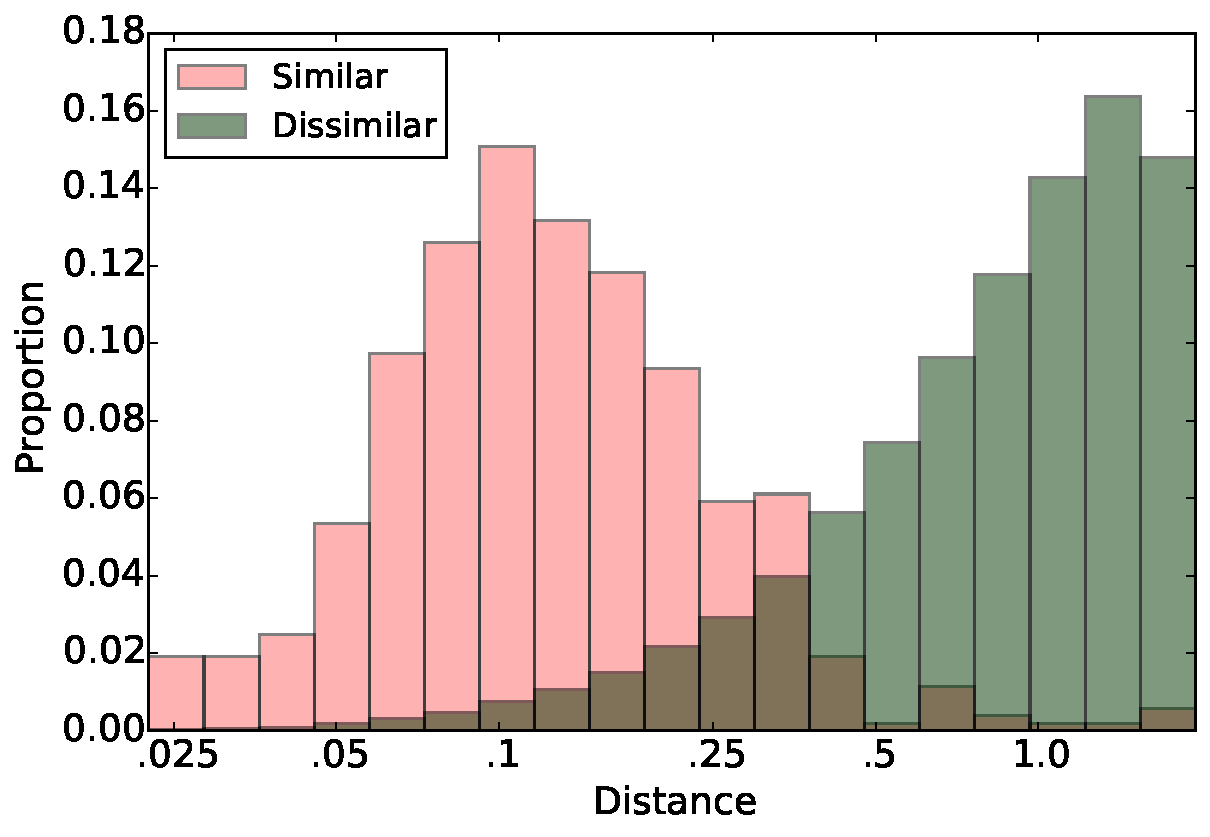
\includegraphics[width=\columnwidth]{distances.pdf}
  \caption{Histograms of embedded distances for positive and negative example pairs in the validation set for our best-performing embedding network.  Note that the x-axis is log-scaled.}
  \label{fig:distances}
\end{figure}

Recall that the goal of this work is to utilize embeddings to speed up large-scale sequence similarity searches by avoiding comparisons to most sequences in a database.
Towards this end, we will utilize embeddings as follows:
First, given a training set of matching sequences, we will train a feed-forward network with attention to embed each sequence in a Euclidean space where similar sequences have a small distance and dissimilar ones have a large distance.
Then, we will utilize this network to pre-compute embeddings for all sequences in a database.
In order to match a query sequence, we will compute the distance between its embedding and all pre-computed embeddings from the database.
Given a test set of correct matches which are known a priori, the effectiveness of this approach can be measured by determining how often the correct match appears in the $N$ entries with the $N$ smallest embedded distances for varying values of $N$.

We will evaluate this approach on the problem proposed in \cite{raffel2015large}.
This work seeks to efficiently match a transcription of a piece of music to a recording of the same piece in a large database of recordings.
The resulting problem boils down to a large-scale subsequence matching problem, where the sequences are particularly long (up to thousands of time steps), the feature dimensionality is relatively high, and the correct match may be a subsequence of the query and vice versa.
These properties make the traditional DTW pruning methods outlined in Section \ref{sec:intro} ill-suited and provide a setting to evaluate completely general-purpose methods like the one proposed in this work.
We will outline the details of the experiment below; for a complete discussion, we refer the reader to \cite{raffel2015large}.

The training set consists of a collection of MIDI files which have been matched to audio files.
MIDI files can be thought of as transcriptions, and can be synthesized in order to obtain an audio recording which is qualitatively similar to the song they are a transcription of.
In \cite{raffel2015large}, the MIDI and audio pairs are also aligned in time to one another using DTW before being used as training data; the system proposed in this work doesn't require sequences which are aligned in time so we skipped this step.
The resulting training set contains 5,536 sequence pairs.

As a representation, we use log-magnitude constant-Q spectrograms \cite{brown1991calculation} of the audio files and MIDI syntheses.
Each constant-Q spectra spanned four octaves, using twelve bins per octave starting from MIDI note C3 (65.4 Hz).
Each frequency bin in all feature sequences was z-scored (standardized) by its mean and standard deviation over the training set.
In \cite{raffel2015large}, using shorter sequences was beneficial so constant-Q spectra were aggregated over estimated beat locations.
The present approach is meant to be able to cope with sequences which may be oversampled in time, so we did not beat-aggregate feature vectors and instead used spectra computed every 46 milliseconds.
All feature analysis and processing was accomplished with \texttt{librosa} \cite{mcfee2015librosa, mcfee2015librosa_scipy}

\begin{figure}[t]
  \centering
  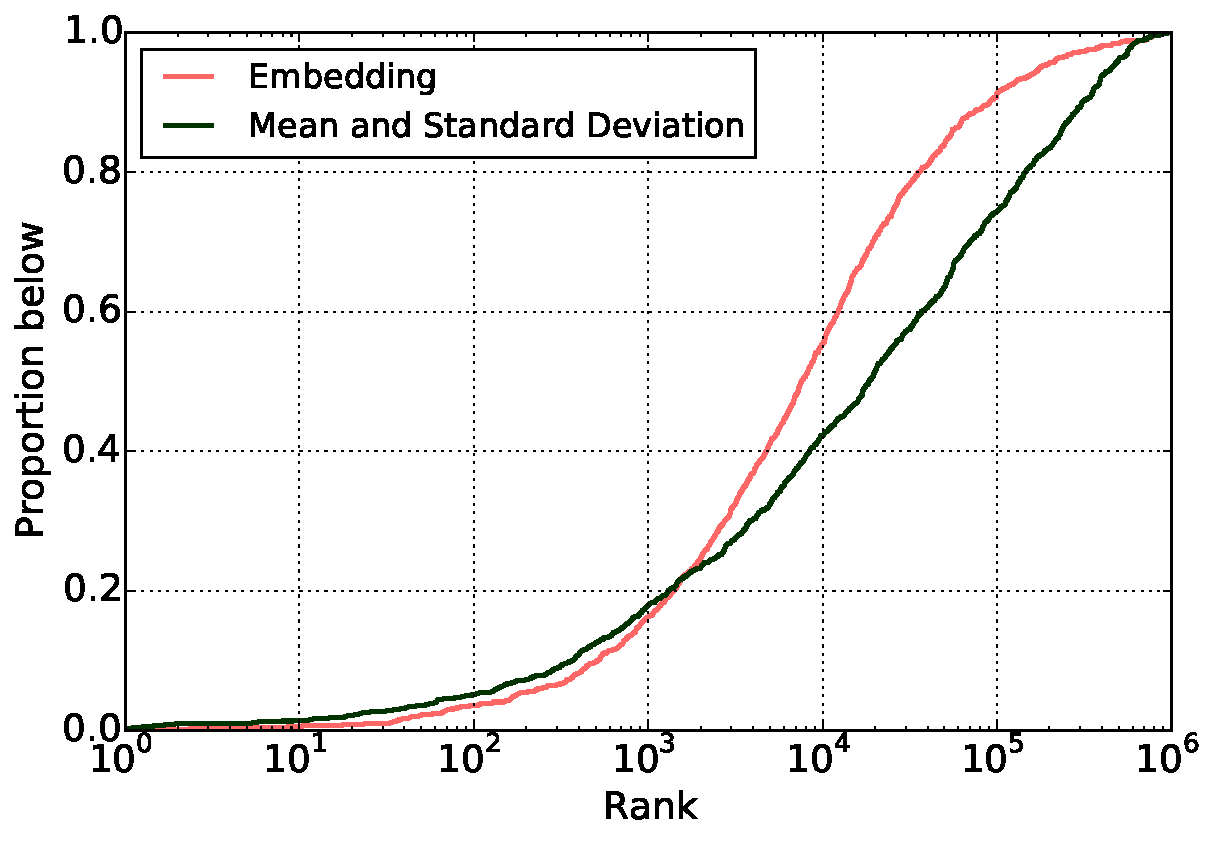
\includegraphics[width=\columnwidth]{ranks.pdf}
  \caption{Proportion of MIDI files in the test set whose correct match appeared below a given rank, based on embedding distances.}
  \label{fig:ranks}
\end{figure}

As a model, we also mimic \cite{raffel2015large} and use a siamese architecture consisting of two parallel convolutional networks followed by two parallel fully-connected networks.
The use of a convolutional ``front end'' allows our model to learn exploit both time and frequency invariances in the constant-Q spectra while reducing the number of model parameters.
The main difference in models is the addition of the attention mechanism proposed in Section \ref{sec:model}, which we place between the convolutional network and the fully-connected network.
In this way, the convolutional network can be seen as transforming a ``raw'' input sequence to a sequence of vectors in a learned representation, which are then aggregated using the attention mechanism and mapped to the embedded space using the fully-connected network.
We used an embedding space dimensionality of 128.

To train the networks, we pass pairs of ``matching'' and ``non-matching'' sequences and utilize a loss function which encourages matching pairs to have similar embeddings and non-matching pairs to have dissimilar ones.
We utilize the same loss function as in \cite{raffel2015large}: Given a pair of positive sequences $X_p, Y_p$ and a set of negative sequences $X_n, Y_n$, we attempt to minimize
$$
\mathcal{L} = \|f(X_p) - g(Y_p)\|_2^2 - \alpha \max(0, m - \|f(X_n) - g(Y_n)\|_2)^2
$$
where $f$ and $g$ are the functions of the two networks being trained, $\alpha$ is a parameter controlling the importance of separating dissimilar pairs, and $m$ is the target separation for dissimilar pairs.
To construct negative pair examples, we simply randomly choose non-matched MIDI/audio sequence pairs from the training set.

\begin{figure*}[htb!]
  \centering
  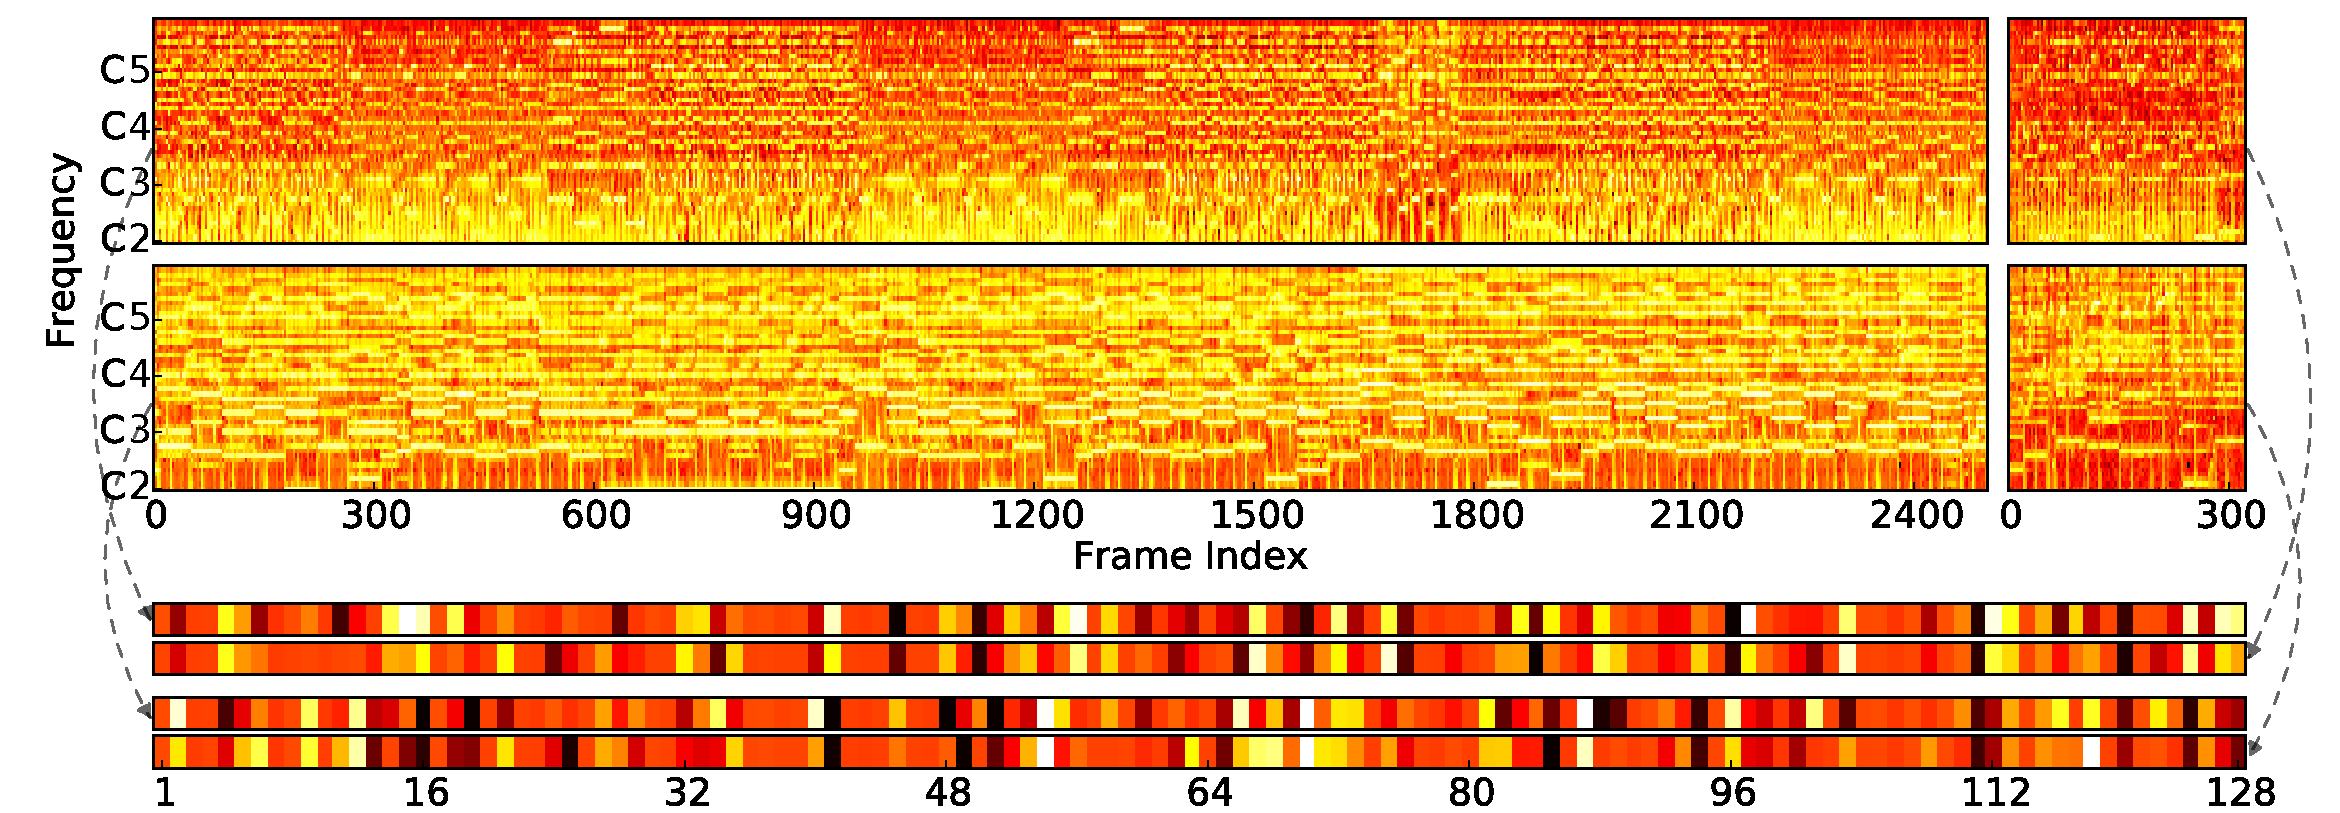
\includegraphics[width=\textwidth]{embeddings.pdf}
  \caption{Embeddings for two pairs of matching sequences from our best-performing system.  The first two rows display pairs of matching constant-Q spectrograms.  For both pairs, the right sequence is a subsequence of the left.  The last two rows show their resulting embeddings.  Dashed arrows denote which embedding corresponds to which sequence.}
  \label{fig:embeddings}
\end{figure*}

As in \cite{raffel2015large} we utilize rectified linear units throughout the network, except on the final output layer which used $\tanh$ units.
All weights were initialized using He et.\ al.'s method \cite{he2015delving} and all biases were initialized to zero.
The networks were optimized with respect to $\mathcal{L}$ using Nesterov's accelerated gradient \cite{sutskever2013importance} with mini-batches of 20 similar and dissimilar pairs.
All sequences were either randomly cropped or padded to the median sequence length in each modality.
Every 100 minibatches, we computed the mean loss $\mathcal{L}$ on a held-out validation set consisting of 10\% of the training set; when it was less than .99 times the previous lowest validation loss, we trained for 500 more minibatches.

To choose hyperparameter settings, we used the Bayesian optimization software package \texttt{spearmint} \cite{snoek2012practical}.
We optimized the number of convolutional and pooling layers, the number of fully-connected layers, the learning rate and momentum, and the loss parameters $\alpha$ and $m$.
We also experimented with using RMSProp \cite{tieleman2012lecture} and adam \cite{kingma2014adam} for optimization and dropout \cite{hinton2012improving} in the fully-connected layers for regularization, but did not find them to be beneficial.
As an objective, we computed the Bhattacharrya coefficient \cite{bhattacharyya1943measure} between the distributions of matching and non-matching pairs in the validation set.
The best-performing network configuration achieved a Bhattacharrya coefficient of .471 and used a single convolutional layer with 16 filters which were 5 time steps wide by 12 semitones tall, one 2x2 max-pooling layer, three fully connected layers (including the final output layer) with 2048 units each, a learning rate of $10^{-4}$, a momentum of 0.997, $\alpha = 0.935$ and $m = 1$.
The validation set distance distributions produced by this network after training can be seen in Figure \ref{fig:distances}.

\section{Results}
\label{sec:results}

Some qualitative intuition about our system's behavior can be gained by inspecting the embeddings resulting from matching and non-matching pairs of sequences.
Embeddings for two different matching sequence pairs from the validation set can be seen in Figure \ref{fig:embeddings}.
Among the four embeddings displayed, the pairs of matched embeddings resulted in Euclidean distances of 0.159 and 0.347, while non-matching pairs had distances of 1.08 and 1.15.
While these distances indicate the appropriate behavior, there are nevertheless some noticeable discrepancies between the embeddings of the matched sequences.

To evaluate our system's performance on the task of pruning large-scale subsequence search, we used it to match a held-out test set of 1,282 MIDI files to entries in the Million Song Dataset (MSD) \cite{bertin2011million}.
Our test set was the same used in \cite{raffel2015large}, for which the correct match in the MSD is known for each MIDI file.
We first computed embeddings of constant-Q spectrograms for all of the short (30 to 60 second) preview recordings of each entry in the MSD provided by 7digital \cite{schindler2012facilitating}.
Then, we computed a constant-Q spectrogram and its embedding for each MIDI file in the test set.
To determine performance, we computed the Euclidean distance between the embedding of each MIDI file and the embeddings of every entry in the MSD and determined how many entries had a distance that was smaller than the correct match.
As a baseline, we performed the same evaluation except using the concatenated mean and standard deviation of the feature dimensions of constant-Q spectrograms as the embedding.
The results can be seen in Figure \ref{fig:ranks}.

To summarize these results, using the proposed method the correct match appeared in the top 100,000 matches 91.3\% of the time using embedding distance and only 74.4\% of the time using the mean and standard deviation of spectrograms.
As noted in \cite{raffel2015large}, matching a single MIDI file to the MSD using dynamic time warping distance would take about three hours; the proposed approach takes about 360 milliseconds per file using a non-optimized Python implementation.
Another way of stating our result, then, is that we can discard 90\% (900,000 entries) of the MSD with 91.3\% confidence using a pruning method which is about 30,000 times faster than the standard DTW-based matching approach.
Compared to the approach proposed in \cite{raffel2015large} which can prune 99\% of the MSD with 95.9\% confidence, it is substantially less accurate, but it is also over 300 times faster.
In addition, our approach is fully general, and was able to achieve good performance on a task that would not be possible using the methods proposed in \cite{rakthanmanon2012searching} or \cite{papapetrou2011embedding}.

While our proposed approach has proven effective, there is room for improvement.
The model may be able to further differentiate between similar and dissimilar sequences if the dimensionality of the embedded space was increased, at the cost of a linear increase in runtime.
Alternatively, choosing negative example pairs more carefully (e.g.\ using the ``harmonic embedding'' approach of \cite{schroff2015facenet}) may further improve discrimination.
Finally, evaluating this approach on more traditional sequence retrieval tasks which allow more stringent assumptions to be made about the correct match would facilitate comparison to existing pruning techniques.
For researchers interested in utilizing and reproducing our results, code is available online.\footnote{\href{http://github.com/craffel/sequence-embedding}{\texttt{http://github.com/craffel/sequence-embedding}}}

\bibliographystyle{IEEEbib}
\bibliography{refs}

\end{document}
